%! TEX root = /home/simon/Documents/Dagbok_MPPHS_2020-2021/main.tex
\subsection{Måndag 2020-08-31}

Nytt läsår, nya mögligheter.

Hade föreläsning i integrationsteorin idag, det är Jeffrey Stein som håller kursen nu. Jag tror det kommer bli hype, han verkar pedagogisk!

Var ute \& sprang med Elin idag. Det kändes rätt bra, lät som att hon var taggad på att springa igen.


\subsection{Tisdag 2020-09-01}

Hade föreläsning i kommutativ algebra idag. Per verkade inte fullt så mossig som folk har beskrivit honom som. + att hans föreläsningar inte krockar med några andra så kanske inte hade varit helt fel att gå på dem ändå.

Hade även föreläsning i standardmodellen idag. Fortfarande osäker på det underliggande materialet, QFTn. Kanske ska gå på hans bakgrundsföreläsningar \& snacka lite med honom om det på hans office hours.

Nu vill jag nog börja planera upp min tid \&så så att jag vet vad jag ska göra när jag kommer till skolan. Imorgon vill jag
\begin{itemize}
    \item Kolla på några av Ferrettis videos (hann fram till \enquote{Gauge Symmetry: Need for a covariant derivative} idag)
    \item Läsa s.\ $x$-$y$ i Steins föreläsningsanteckningar (TODO: kolla hur långt han tänker hinna nästa lektion. DET STOD \enquote{9/3: F 1.3,4 and JJ 3.7 and Theorem 3.10} PÅ CANVAS)
\end{itemize}

Fick tillbaka subben idag \&så, fick 35p så det var inte superhype. Kollade lite på rättningen \& hade fått 3/15p på en uppgift där man bara skulle räkna på hur långt en lepton behövde färdas innan det var \SI{50}{\percent} sannolikhet att den bytte smak. Fattar inte hur jag kunde gjort så fel, det känns ju som en fett lätt uppgift. Aja, får grotta ner mig i den uppgiften \& sen alla relativistiska beräkningar inför nästa tent.


\subsection{Onsdag 2020-09-02}

TODO: installera \href{https://awesomeopensource.com/project/lervag/vimtex?categoryPage=4}{\color{blue}vimtex}. $\checkmark$

Installerade neovim (\verb|nvim|) med vim-plug som package manager. Sen följde jag en \href{https://yufanlu.net/2018/09/03/neovim-python/}{\color{blue}guide} för att få rätt highlighting \& code completion \& debugging etc i vim när jag skriver python-kod. För att det allt ska fungera måste man även ha installerat
\begin{itemize}
    \item jedi for code completion: \verb|pip install jedi|
    \item flake8 for code linting: \verb|pip install flake8|
    \item autopep8 for code formatting: \verb|pip install autopep8|
\end{itemize}
Jag lade även in en hotkey (f5) i vim för att köra .py-script genom att lägga till\\
\texttt{
    autocmd FileType python map <buffer> <F5> :w<CR>:exec '!python3'\\ shellescape(@\%, 1)<CR>\\
    autocmd FileType python imap <buffer> <F5> <esc>:w<CR>:exec '!python3'\\ shellescape(@\%, 1)<CR>
}\\
i \verb|init.vim|.

Nästa steg är att följa den \href{https://yufanlu.net/2018/09/03/neovim-latex/}{\color{blue}guiden} för att få samma funktionalitet i .tex-filer. Jag gorde det \& installerade vimtex. Dock fungerar inte code completion... aja, får kolla mer på det sen. Man använder
\begin{itemize}
    \item \verb|:VimtexCompile| För att starta kontinuerlig kompilering (varje gång vi sparar)
    \item \verb|:VimtexView| För att öppna den kompilerade pdfen
    \item \verb|:VimtexErrors| För att visa alla errors.
\end{itemize}
Man modifierar \verb|init.vim|-filen (där står det vilka plugins man använder etc) genom\\ \verb|gedit ~/.config/nvim/init.vim|. Jag lade till ett autocomplete plugn som man anvnder genom att bläddra mellan förslag med tab \& shift-tab.


\bigskip

Allmän fundering: kanske najjs att använda verbatim, \verb+\verb||+, för att displaya kod.

\bigskip

\verb|polynom|-paketet gör polynomdivision åt mig:
\begin{center}
    \polylongdiv{x^3 - 7 x - 6}{x + 1}
\end{center}


\subsection{Torsdag 2020-09-03}

Höll i rövningen imorse. Det var fett hetsigt i början för zoom fungerade inte, tydligen, eftersom William hade skapat alla fyra mötena, kunde inte alla mötena vara igång samtidigt. Så det tog lite tid att fatta vad som var fel \& sen skapa ett nytt rum \& skicka ut till folk.

\subsection{Fredag 2020-09-04}


Bra features i vimtex:
\begin{itemize}
    \item Move between section boundaries with \verb|[[|, \verb|[]|, \verb|][|, and \verb|]]|
    \item Delete the surrounding command, environment, or delimiter with \verb|dsc|, \verb|dse|, \verb|ds$|, or \verb|dsd|
    \item Change the surrounding command, environment, or delimiter with \verb|csc|, \verb|cse|, \verb|cs$|, or \verb|csd|
    \item Toggle between e.g. \verb|()| and \verb|\left(\right)| with \verb|tsd|
    \item Close the current environment/delimiter in insert mode with \verb|]]|
\end{itemize}
Speciellt \verb|dse|, \verb|cse|, \& att avsluta nuvarande miljö med \verb|]]|.



\bigskip

Ferretti snackade om \href{http://feynrules.irmp.ucl.ac.be/}{\color{blue}FeynRules} som är ett Mathematica-paket som räknar ut Feynmanregler för olika kvantfältteorier. Han sa att det var rätt lätt:
\begin{figure}[H]
    \centering
    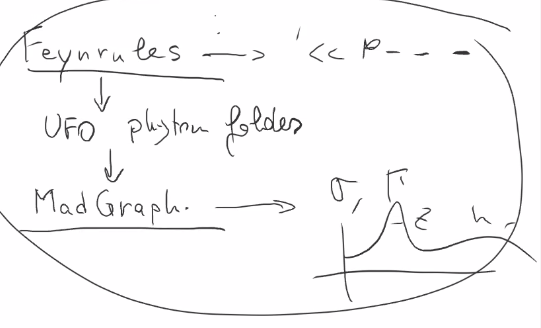
\includegraphics[width=0.7\textwidth]{pics/ferretti_on_FeynRules.png}
\end{figure}

Jag testar ladda ned dagboken \& köra lite lokalt ett tag så  jag kan vänja mig vid vim. Jag testar ladda ned dagboken \& köra lite lokalt ett tag så  jag kan vänja mig vid vim.

\subsection{Lördag 2020-09-05}

Jag tror att jag har lyckas köra latex nu från vim :). Dock kunde jag ju välja TeX Live 2017 i Overleaf \& sen importera aligned-overset-paketet manuellt för att undvika errors. Det kan jag inte göra nu så måste helt skippa bibtex. Känns aningens ovärt, men liksom, vrf skulle jag behöva bibtex i min dagbok?

Jag löste det så att VimTeX kompilerar \verb|main.tex| om man sparar t.ex.\ \verb|LP1/v1.tex|. Man måste skriva \verb|%! TEX root = /home/simon/Documents/Dagbok_MPPHS_2020-2021/main.tex| på första raden i \verb|LP1/v1.tex| för att VimTeX ska fatta vilken som är main-filen.

TODO: kolla upp vad det där vim-temat var som såg ballt ut som du såg på reddit. Det var typ Marianne eler ngt sånt. \checkmark\\
Den hette \emph{Miramare}. Protip är att komma ihåg att köra \verb|:PlugUpdate|.

TODO: ladda ned Meals on Wheels eller ngn annan najjs Jackie Chan-film.

\bigskip

Jag kan skriva dagbok från telefonen nu \&så via ssh.


\subsection{Söndag 2020-09-06}

Läser lite integrationsteori idag inför kommande vecka.

Vi testar några nya kommandon:
\begin{align}
	A = \Union_{i = 1}^\infty A_i \quad A = \Intersection_{i = 1}^\infty A_i\\
	A = B \union C \quad A = B \intersection C.
\end{align}

